
La detección de muones en este proyecto es realizada mediante un detector de partículas inspirado en los detectores sTGC del proyecto ATLAS, en CERN. La sigla significa ''small Thin Gap Chamber", y forman parte de un espectrómetro de muones que permite conocer momento y trayectoria de estas partículas. Los muones proveen de información importante para la reconstrucción de eventos asociados a colisiones de partículas.

\begin{figure}[h]
	\centering
	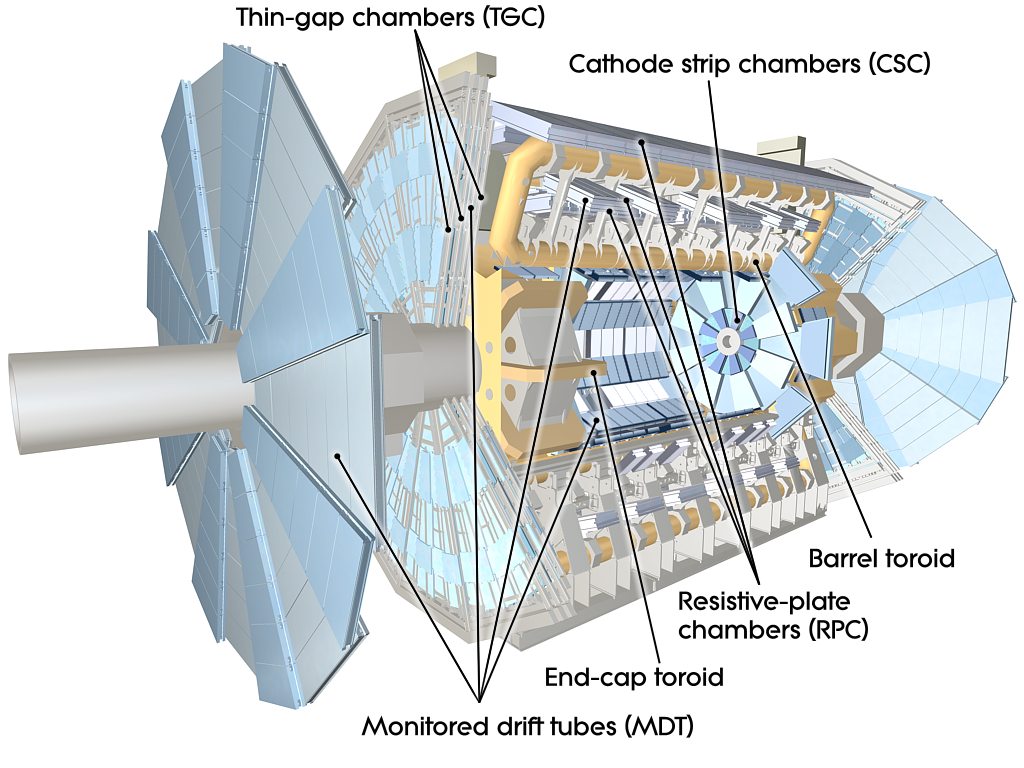
\includegraphics[scale=0.3]{atlas-muon-spectrometer-layout.png}
	\caption{Diagrama del espectrómetro de muones en el proyecto ATLAS\cite{AtlasMuonDiagram}.}
	\label{img:atlas-layout}
\end{figure}

\newpage
\begin{figure}[h]
	\centering
	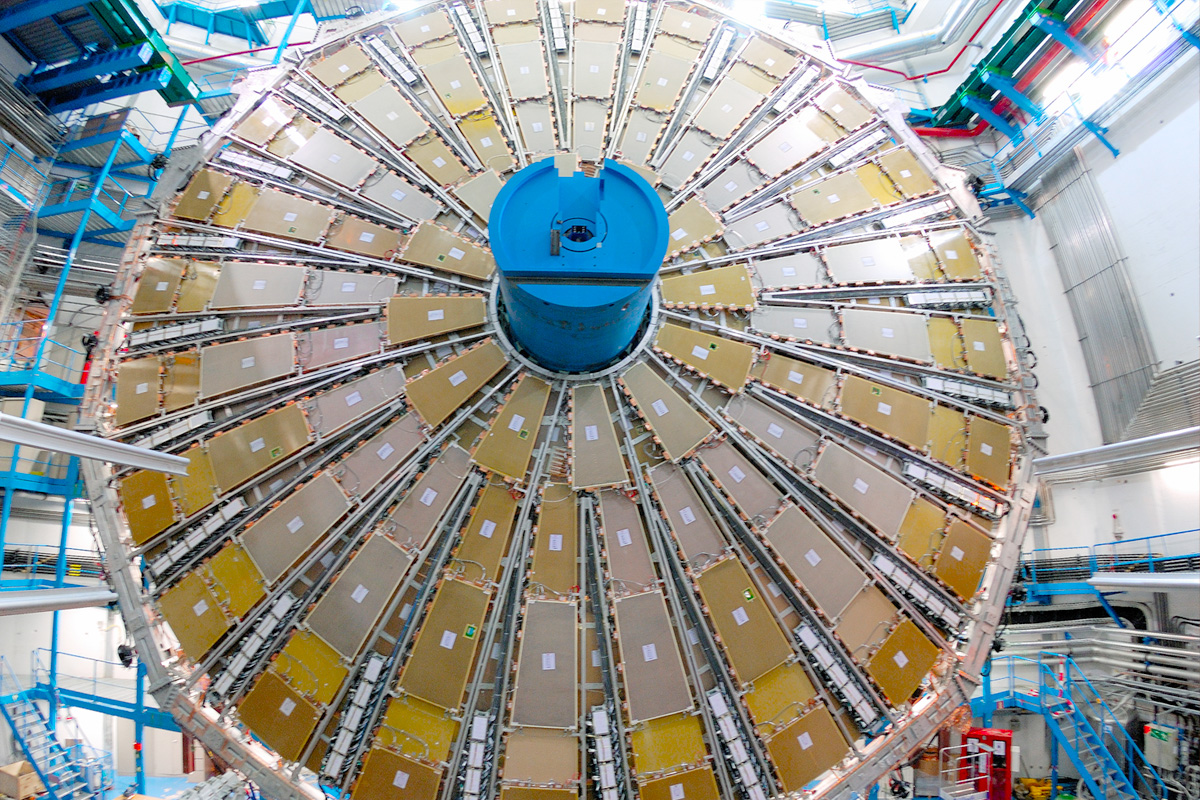
\includegraphics[scale=0.3]{atlas-muon-tgc.jpg}
	\caption{Fotografía del los detectores sTGC en el espectrómetro de muones del proyecto ATLAS\cite{AtlasMuonSpect}.}
	\label{img:atlas-tgc}
\end{figure}

\begin{figure}[h]
	\centering
	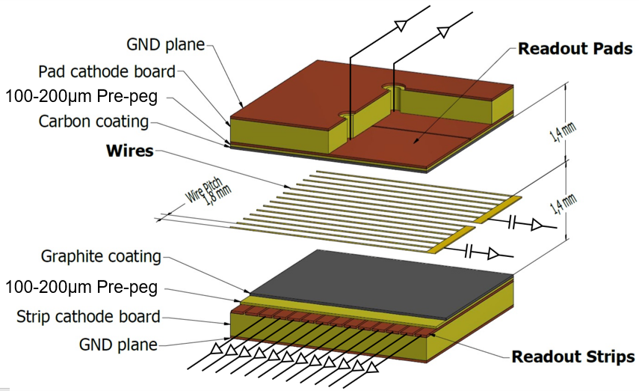
\includegraphics[scale=0.7]{tgc-structure.png}
	\caption{Estructura interna de un detector TGC\cite{Chapman2014}.}
	\label{img:stgc-structure}
\end{figure}

\begin{figure}[h]
	\centering
	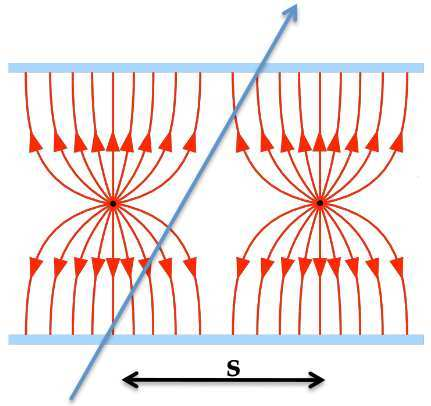
\includegraphics[scale=0.3]{stgc-transversal.png}
	\caption{Lineas de campo eléctrico observadas en un corte transversal de los cables y cátodos del detector. Los cátodos se ilustran en celeste, los cables se representan en negro, y las lineas de campo corresponden a las flechas de color rojo\cite{GEMTracker}.}
	\label{img:stgc-field}
\end{figure}

\newpage
\subsection*{Estructura}

	Un TGC está compuesto por dos planos de grafito (cátodos), con múltiples cables en medio (ánodos). Recubriendo el exterior de ambos cátodos se ubican capas aislantes que los separan de zonas conductoras. Estas zonas son llamadas ''\textit{strips}´´ en la cara superior y ''\textit{pads}´´ en la cara inferior del detector. Los cables se encuentran orientados perpendicularmente respecto a los \textit{strips}.
	
	Al interior del detector, entre los planos de grafito, se infiltra un gas compuesto por dióxido de carbono y n-pentano. Mediante la aplicación de alto voltaje, se genera un campo eléctrico entre ánodos y cátodos. El paso de muones a través del detector genera entonces la ionización del gas y la liberación de electrones, los cuales son captados por los cables del detector gracias al campo eléctrico.
	
	El flujo de electrones en el gas ionizado genera pulsos de corriente en los cables, produciendo a la vez diferencias de potencial en los cátodos. Estos interactúan con los \textit{pads} y \textit{strips} en el exterior, en los cuales aparecen pulsos de corriente con polarizad inversa respecto a los cables.
	
	La amplitud de los pulsos generados en el detector será mayor en torno a la zona del evento ionizante y menor en zonas lejos de ella. Esto permite relacionar la posición y energía de la partícula con las amplitudes de los pulsos en cada \textit{strip} o cable.

\subsection*{Detector sTGC Utilizado}
	En ATLAS se leen señales provenientes de cátodos y ánodos a la vez. Esto permite trazar coordenadas de posición para cada evento, ya que los \textit{strips} son perpendiculares a los cables. En este proyecto de titulación se leerán solo las señales provenientes de los \textit{strips}, por los que solo se estaría midiendo un eje de posición. 
	
	Para agregar un eje adicional, se reemplazan los \textit{pads} de la cara inferior por \textit{strips} perpendiculares a los del plano contrario. Así se logra tener información bidimensional del paso de una partícula leyendo solo las señales provenientes de \textit{strips}.
	
	\begin{figure}
		\centering
		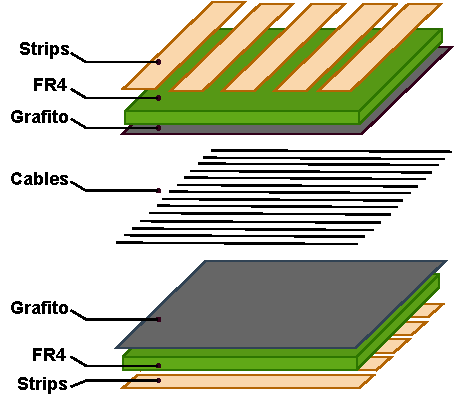
\includegraphics[scale=1]{stgc-mini-estructura}
		\caption{Estructura interna de un detector sTGC adaptado para este proyecto de titulación. El gas es contendio entre ambas capas de grafito. Los recubrimientos de grafito corresponden a los cátodos, mientras que los cables internos corresponden a los ánodos.}
		\label{img:stgc-mini-estructura}
	\end{figure}
	
	
	\begin{figure}
		\centering
		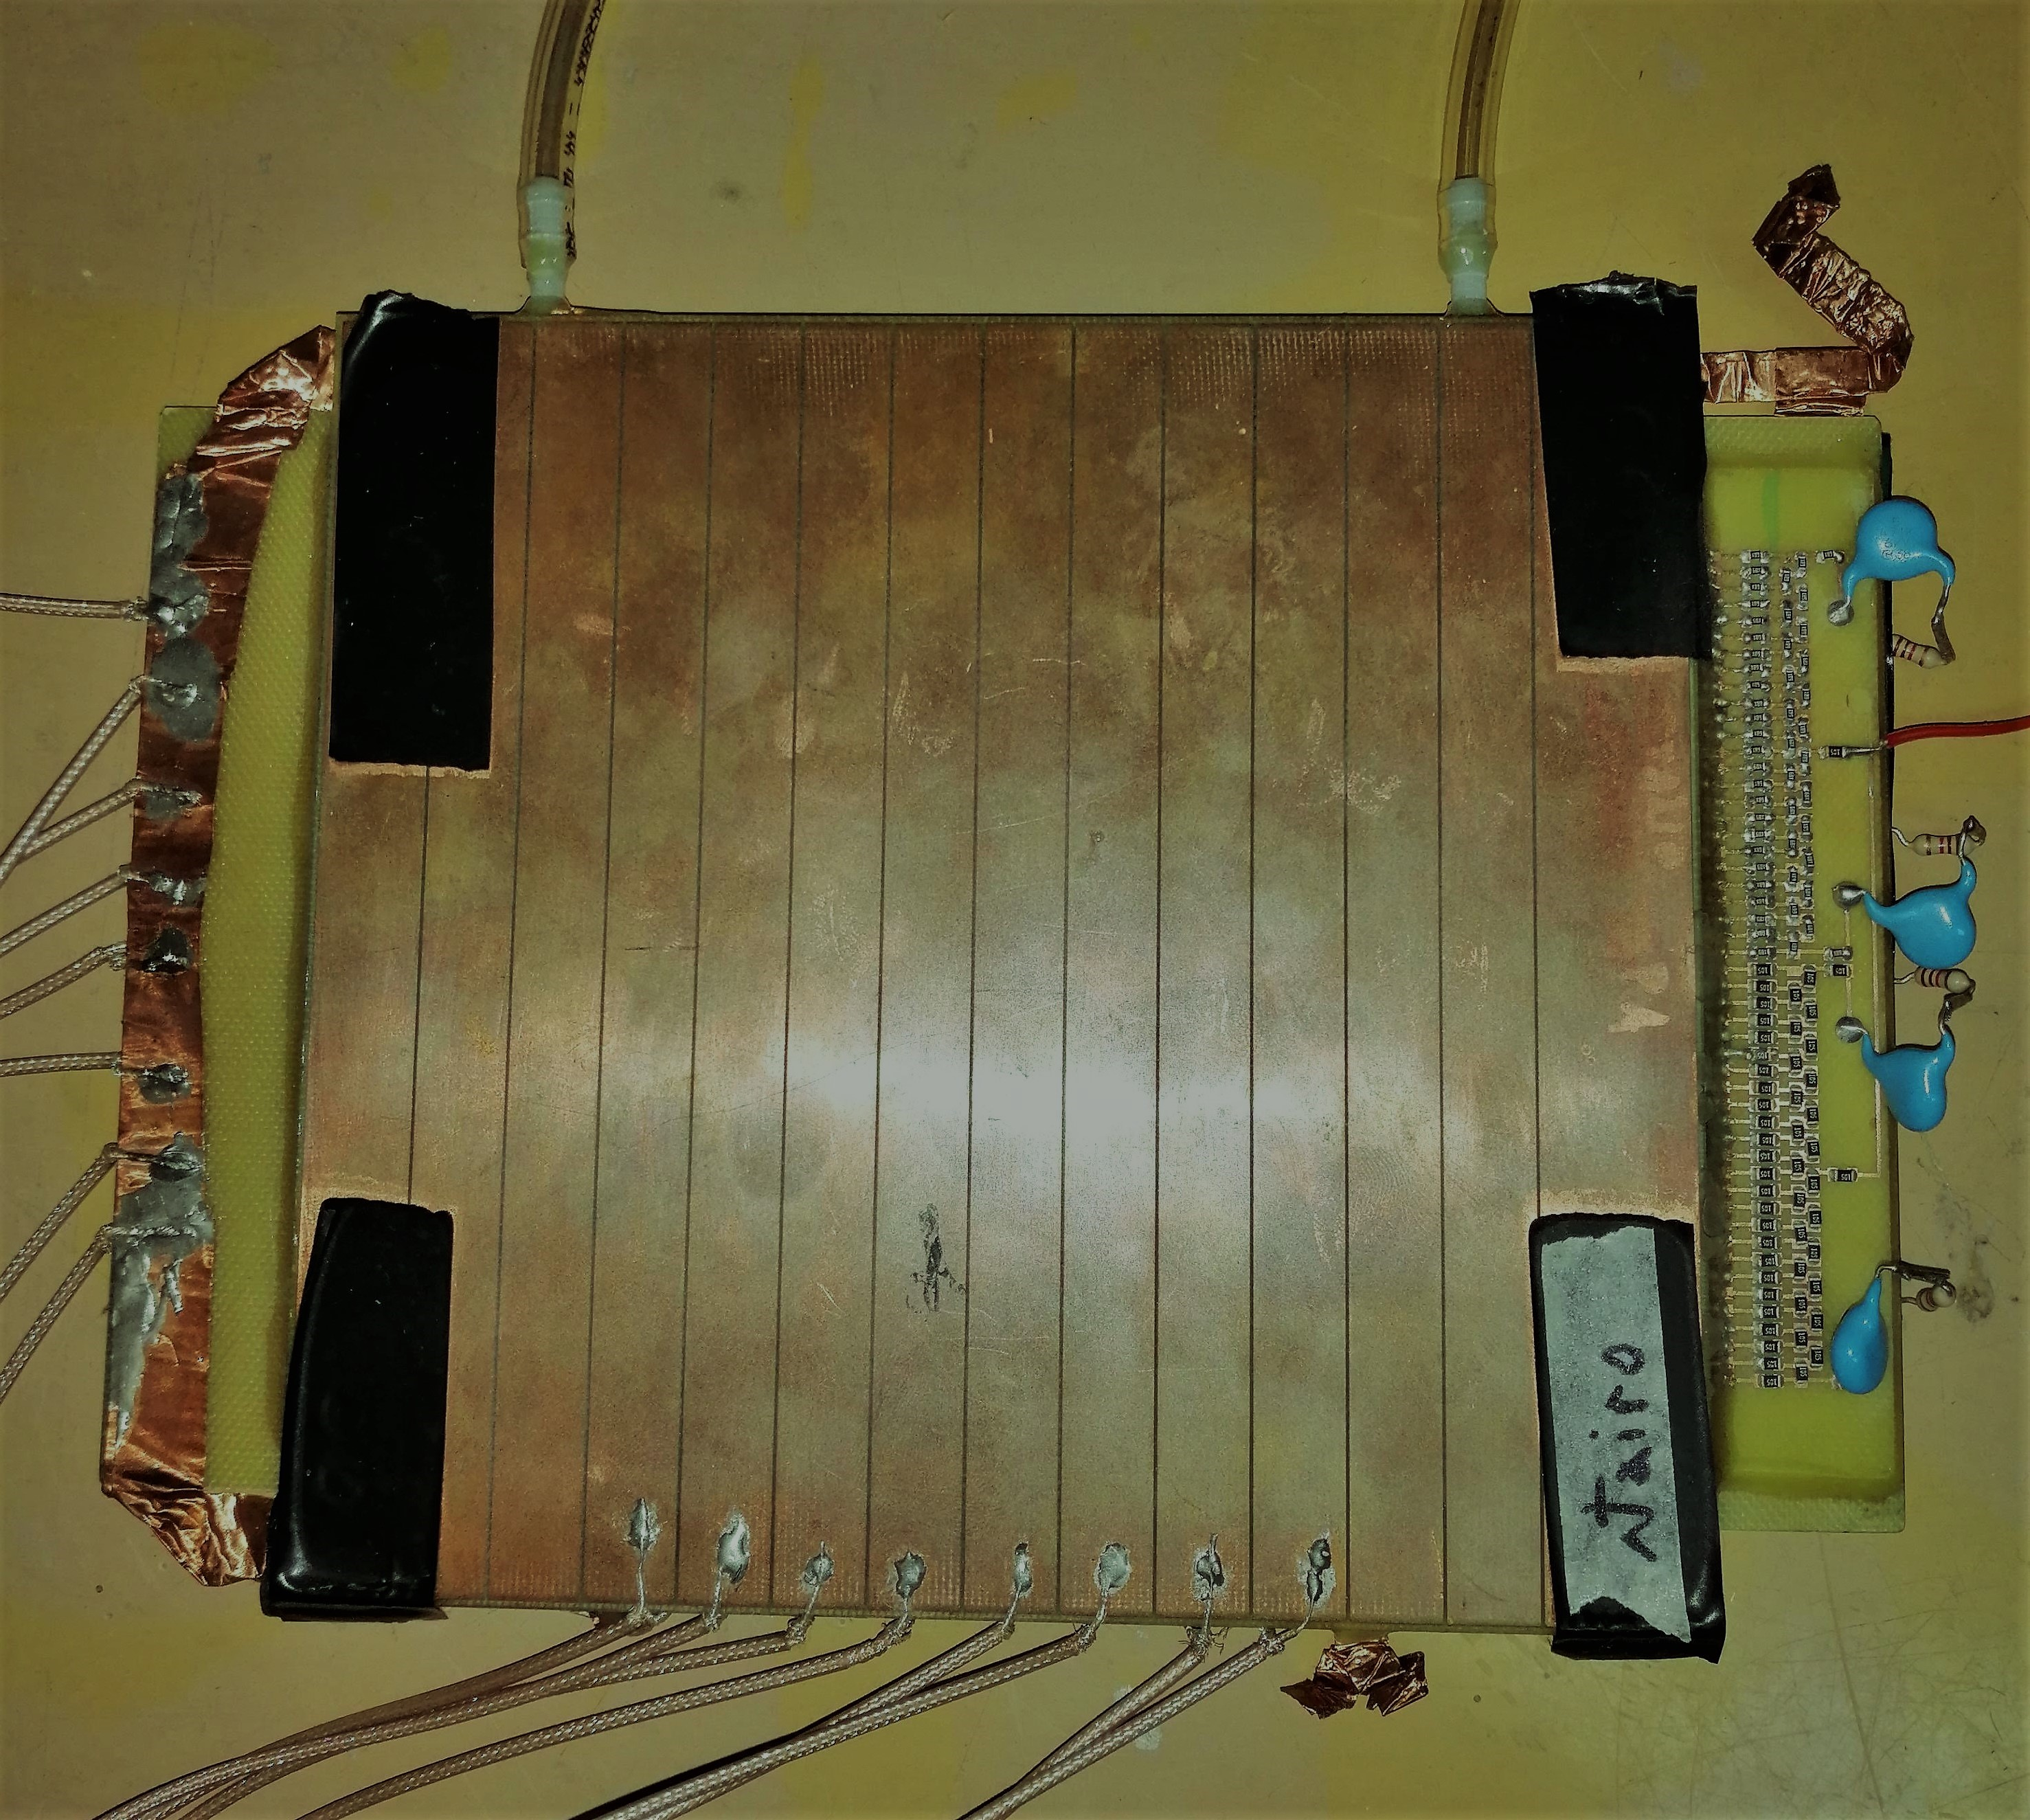
\includegraphics[scale=0.09]{mini-stgc.jpg}
		\caption{Vista superior del detector utilizado. Arriba se observan tubos para el flujo de gas. Abajo se ubican 8 cables coaxiales conectados a los \textit{strips} centrales de una cara del detector. A la izquierda están situados los otros 8 cables correspondientes a los \textit{strips} de la cara inferior. En el costado derecho se observa una red resistiva ponderadora para la lectura de los cables internos del detector, los cuales no serán utilizados en este proyecto.}
		\label{img:foto-mini-stgc}
	\end{figure}
	
	En particular, el detector utilizado cuenta con 8 \textit{strips} útiles por lado, de 10 centímetros largo y 1 centímetro cada uno. Se utilizan 3000 $V_{DC}$ entre cátodos y ánodos para generar el campo eléctrico, limitando la corriente a 50uA. El gas en su interior puede ser dióxido de carbono puro, con el compromiso de generar mayor cantidad de descargas no asociadas a muones.

%pruebas, gráficos, entradas y salidas, triggers, plásticos, fuentes radioactivas